\documentclass[xetex,mathserif,serif]{beamer}

\usepackage[export]{adjustbox}
\usepackage{listings}
\usepackage{color}
\usepackage{fontspec}
\usepackage{multicol}

%\usetheme{Darmstadt}
%\usecolortheme{beetle}

\usetheme{Madrid}
\useoutertheme{miniframes} % Alternatively: miniframes, infolines, split
\useinnertheme{circles}

\definecolor{UBCblue}{rgb}{0.29412, 0.2745, 0.53334} % UBC Blue (primary)

\usecolortheme[named=UBCblue]{structure}
%\usecolortheme[named=Mahogany]{structure} % Sample dvipsnames color
\usepackage{graphicx}
\makeatletter
\providecommand{\bigsqcap}{%
  \mathop{%
    \mathpalette\@updown\bigsqcup
  }%
}
\newcommand*{\@updown}[2]{%
  \rotatebox[origin=c]{180}{$\m@th#1#2$}%
}
\makeatother




\title [Apstraktna interpretacija]% (optional, only for long titles)
{Apstraktna interpretacija u modernim kompajlerima}
\subtitle{Seminarski rad u okviru kursa Metodologija stručnog i naučnog rada}
\author[\quad Demonja, Maksimović, Crnobrnja \quad] % (optional, for multiple authors)
{O.~Demonja, S.~Maksimović i M.~Crnobrnja}
\institute% (optional)
{
  Matematički fakultet\\
  Univerzitet u beogradu
}
\date % (optional)



\begin{document}
  \frame{\titlepage}
  
  \begin{frame}
    \frametitle{Uvod}
	    \framesubtitle{Pojmovi}
		\begin{center}
		\begin{itemize}
			\item \textbf{Apstraktna interpretacija} je tehnika za automatsku statičku analizu programa
			\item Zamena preciznih elemenata sa manje detaljnim apstrakcijama
			\item Apstrakcija dovodi do gubitka sigurnih informacija što dovodi do nemogućnosti dovođenja zaključaka za sve programe
			\item Otkrvanje greški nastalih tokom izvršavanja programa 
				\begin{itemize}
					\item deljenje sa 0
					\item razna prekoračenja
					\item mrtve petlje
					\item ...
				\end{itemize}
		\end{itemize}
	\end{center}
  \end{frame}  
  
  \begin{frame}
    \frametitle{Apstraktna interpretacija}
	    \framesubtitle{Problem koji se rešava}
		\begin{center}
			\begin{itemize}
			\item {Način transporta} \only<2-4> {(mapa je apstraktna reprezentacija)}
			\begin{itemize}
				\item avionom
				\item voz
				\item pešaka
			\end{itemize}

			\pause			
			\pause			
			
	        \item $a_{+} \times a_{-}$ \only<4> {(pravilo znaka pri množenju)}\\
    	    {\color{cyan} $\times$ množenje, $a_{+}$ pozitivan, $a_{-}$ negativan broj}
    	\end{itemize}

   		 \begin{itemize}
     		\item $0 \times a_{+} = 0 \times a_{-} = a_{+} \times 0 = a_{-} \times 0 = 0$ \\
     		$a_{+} \times a_{+} = a_{-} \times a_{-} = a_{+}$ \\
     		$a_{+} \times a_{-} = a_{-} \times a_{+} = a_{-}$
    	\end{itemize}
	\end{center}
  \end{frame}    
  
  
  
%\begin{frame}
%    \begin{itemize}[<+->]
%        \item A
%        \item B
%        \item C
%    \end{itemize}

%    \pause  % double pause here

%    Some text.
%\end{frame}
  
  
\begin{frame}
	\frametitle{Apstraktna interpretacija}
	\framesubtitle{Problem koji se rešava}
	\begin{multicols}{2}
	\begin{itemize}
     \item $a_{+} \pm a_{-}$ \\
     {\color{cyan} $\pm$ sabiranje i oduzimanje}
     
     \item $0 \pm a_{-} = a_{-} \pm 0 = a_{-,0} $ \\
      $a_{+} \pm a_{+} = a_{+}$ \\
      $a_{-} \pm a_{-} = a_{-}$ \\
    
    \pause 
     
     \item $a_{+} \pm a_{-} = ??$ \\
      $a_{-} \pm a_{+} = ??$
     
	\pause     
     
     \item $a_{0} = \{0\}$ \\
      $a_{+} = \{n \mid n > 0\}$ \\
      $a_{-} = \{n \mid n < 0\}$
    
    \end{itemize}
    \end{multicols}

	\pause

	\begin{itemize}
		\item $s \pm a = a \pm s = a \pm a = a \quad \text{gde je s} \in \{0, -, +\}$
	\end{itemize}	       
\end{frame}  


\begin{frame}
	\frametitle{Apstraktna interpretacija}
	\framesubtitle{Korišćenje u računarstvu}
	\begin{itemize}
     \item Analiza strogosti:
     \begin{itemize}
		\item Optimizacija lenjih funkcionalnih programa identifikujući parametre koji mogu biti prosleđeni po vrednosti   
		\only<3> {\item {\color{red} Analiza neće uspeti da detektovati neke parametre}}   
     \end{itemize}
     
     \item Analiza menjanja u mestu:
        \begin{itemize}
			\item Određivanje mesta u programu gde je sigurno uništiti objekat  
			\only<3> {\item {\color{red} Analiza će kopirati neke objekte koji su mogli biti uništeni}} 
    	 \end{itemize}     	
     \item Analiza moda:
        \begin{itemize}
			\item Brži rad Prologa prepoznavanjem ulazno-izlaznih promenljivih 
			\only<3> {\item {\color{red} Analiza neće uspeti detektovati sve ulazno-izlazne promenljive}} 
    	 \end{itemize}

	\pause
	\item Optimizacije zasnovane na apstraktnoj interpretaciji mogu \textbf{preskočiti neke optimizacije}      
      
    \end{itemize}
\end{frame} 




  
  
  \begin{frame}
    \frametitle{Formalizacija}
	    \framesubtitle{Skupovi konkretnih i apstraktnih stanja}
		\begin{center}
			\begin{itemize}
				\item $v \in V$ skup konkretnih stanja; \pause $v_{1} \rightsquigarrow v_{2}$ \emph{relacija} prelaska \pause
				%\item $... \rightsquigarrow v_{n} \rightsquigarrow v_{n}$ zaustavljanja programa
				\item $l \in L$ prostor svojstava; \pause $l_{1} \rightarrow l_{2}$ \emph{funkcija} prelaska \pause
				\item $\sqsubseteq \; \; \subset \; L \times L$ relacija poretka nad $L$ \pause
%				\begin{itemize}
%					\item $a \sqsubseteq a$ refleksivnost
%					\item $a \sqsubseteq b \wedge b \sqsubseteq a \implies a = b$ antisimetričnost
%					\item $a \sqsubseteq b \wedge b \sqsubseteq c \implies a \sqsubseteq c$ tranzitivnost
%				\end{itemize}
				\item $( L, \bigsqcup, \bigsqcap)$ potpuna mreža \pause
				\begin{itemize}
					\item $\forall l_0 \in L^{\prime} \; \; l_0 \sqsubseteq \bigsqcup_{l \in L^{\prime}} l$ %\pause
					\item $\forall l_0 (\forall l \in L^{\prime} \; l \sqsubseteq	l_0) \implies \bigsqcup_{l \in L^{\prime}} l \sqsubseteq l_0 $ \pause
					\item analogno za $\bigsqcap_{l \in L^{\prime}} l$ ... \pause
				\end{itemize}
				\item $\rho \subset V \times L$ relacija ispravnosti
				\begin{figure}
					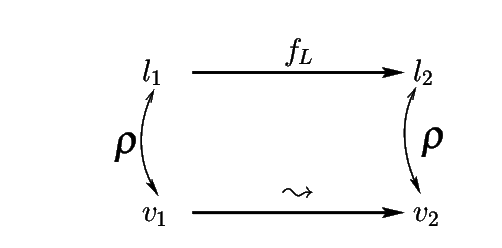
\includegraphics[scale=0.3,left]{Rho.png}
				\end{figure}
			\end{itemize}
		\end{center}
  \end{frame}
  \begin{frame}
    \frametitle{Formalizacija}
    \framesubtitle{Fiksne tačke}
	\begin{center}
		\begin{itemize}
			%\item $l \sqsubseteq \gamma(\alpha(l))$ \pause
			\item $x = f_{L}(x)$, \pause čine potpunu mrežu ukoliko je $f_{L}$ monotona.\pause
			\item $f^{0}_{L}(\bot) = \bot, \quad f^{n+1}_{L}(\bot) = f_{L}(f^{n}_{L}(\bot))$ \pause
			\item $\bigsqcup \{ \: f^{n}_{L}(\bot)\: \}_{n \in \mathbb{N}}$ je najmanja fiksna tačka \pause
			\begin{itemize}
				\item {\color{red} nepraktično za izračunati }			\pause
			\end{itemize}
			\item uvodimo prostor $M$ i \emph{Galoaovu vezu}  $\langle L, \alpha, \gamma, M \rangle$
		\end{itemize}
		\begin{figure}
			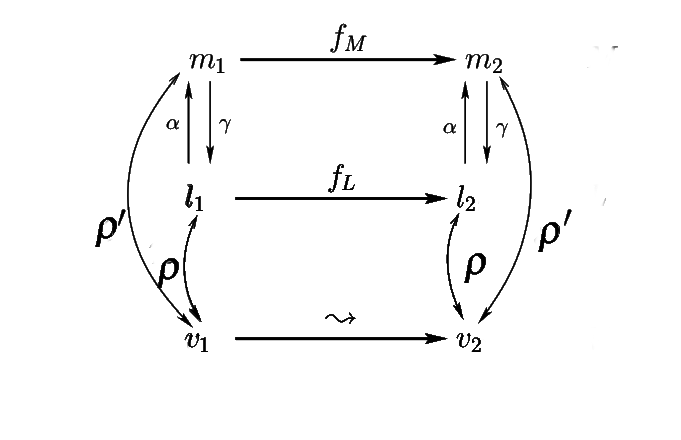
\includegraphics[scale=0.3,left]{Rho_prime.png}
		\end{figure}
		\end{center}
  \end{frame}
  %
  \begin{frame}

    \frametitle{Formalizacija}
    \framesubtitle{Operator proširenja}
    \begin{center}
    	\begin{itemize}
    		\item $\nabla : L \times L \rightarrow L$ ubrzava konvergenciju \pause
    		\item $\forall x,\! y \; x \sqsubseteq x \nabla y, y \sqsubseteq x \nabla y$ \pause
    		\item $x^{\prime}_{0} = y_{0}, \; x^{\prime}_{n} = x^{\prime}_{n-1} \nabla y_{n}$ tada $(x^{\prime}_{n})_{n}$ konvergira u konačnom broju koraka \pause
    	\end{itemize}
    	$$
			f^{n}_{\nabla} = 
			\begin{cases}
			\bot,            								  
				& 	\text{za} \quad n = 0 \\
			f^{n-1}_{\nabla} 							      
				& \text{za} \quad n > 0 \quad \text{i} \quad f_{L}(f^{n-1}_{\nabla}) \sqsubseteq f^{n-1}_{\nabla} \\
			f^{n-1}_{\nabla} \nabla f_{L}(f^{n-1}_{\nabla})  
				& \text{inače}
			\end{cases}
		$$
		\pause
		\begin{itemize}
			\item $lim_{n \rightarrow \infty }f^{n}_{\nabla} \quad$ --- \quad {\color{green} aproksimira najmanju fiksnu ta\v cku}
		\end{itemize}
	\end{center}
  \end{frame}
  \begin{frame}
    \frametitle{Primeri}
    \framesubtitle{Uvod}
    \begin{center}
		\begin{itemize}
			\item Uglavnom intraproceduralna apstraktna interpretacija - vr\v si se za svaku funkciju posebno
			\begin{itemize}
				\item Tra\v zenje konstantnih varijabli
				\item Dereferenciranje null pokaziva\v ca
				\item Inicijalizacija promenljivih koje se kasnije koriste
				\item \emph{lock/unlock, fopen/fclose}
			\end{itemize}
			\item Primer na problemu \emph{propagacije konstanti}
			\begin{itemize}
				\item Prolaz kroz funkciju koriste\v ci apstraktne vrednosti kao ulaz 
				\item Apstraktna vrenost predstavlja skup konkretnih vrednosti
				\item Kada imamo grananje, krenimo put obe grane
				\item Gde imamo spajanje, spajamo izlaz iz obe grane
			\end{itemize}
		\end{itemize}
	\end{center}
  \end{frame}
  \begin{frame}
	\frametitle{Primeri}
    \framesubtitle{Graf kontrole toka, CFG}
	\begin{center}
   		\begin{multicols}{2}
%   		\begin{lstlisting}[basicstyle=\tiny]
			\lstinputlisting[language=C++, basicstyle=\footnotesize]{snippets/ex1.cpp}
%		\end{lstlisting}
    		\begin{figure}
				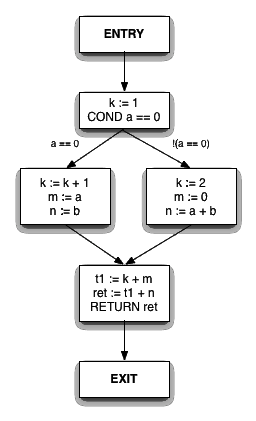
\includegraphics[scale=0.4,right]{Treehydra-cfg.png}
			\end{figure}
		\end{multicols}
	\end{center}
  \end{frame}
  \begin{frame}
    \frametitle{Primeri}
    \framesubtitle{Karakteristike apstraktne interpretacije}
	\begin{center}
		\begin{itemize}
			\item Ta\v cnost i pouzdanost
				\begin{itemize}
					\item Stati\v cka analiza nije savr\v sena, moramo praviti kompromis
					\item Vr\v senje stro\v zijih provera, prijavljivanje la\v znih pozitiva
					\item Bla\v ze provere, \v sansa da nam promaknu neke gre\v ske
				\end{itemize}
			\item Cena
				\begin{itemize}
					\item Algoritmi u najgorem slu\v caju eksponencijalne slo\v zenosti
					\item  {\color{green} Test se izvr\v sava direktno nad kodom}
					\item {\color{red} Dosta se sporije vi\v si od procesa prevo\dj{}enja}
				\end{itemize}
		\end{itemize}
	\end{center}
  \end{frame}
  \begin{frame}
    \frametitle{Zaklju\v cak}
	\begin{center}
		\begin{itemize}
 			\item Veoma zanimljiva tema \pause
			\item Primarno se koristi za stati\v cku verifikaciju \pause
			\item Uglavnom se ne koristi se u kompajlerima \pause
			\begin{itemize}
				\item $\dots$ {\color{green} ali ima puno potencijala}
			\end{itemize}
			
		\end{itemize}
	\end{center}
  \end{frame}
    \begin{frame}
    \frametitle{Literatura}
	\begin{center}
	\end{center}
  \end{frame}
% etc
\end{document}